
\documentclass[]{beamer}
\usetheme{metropolis}
 \usepackage[utf8]{inputenc}
 \usepackage[french]{babel}
 %\usepackage[T1]{fontenc}


\usepackage{listings}

 \usepackage{hyperref}
\hypersetup{
    colorlinks=true,
    linkcolor=black,
    filecolor=magenta,      
    urlcolor=cyan,
}

 \lstset{
 frame=tb,
  language=python,
  aboveskip=3mm,
  belowskip=3mm,
  showstringspaces=false,
  columns=flexible,
  basicstyle={\footnotesize\ttfamily},
  numbers=none,
  numberstyle=\tiny\color{gray},
  keywordstyle=\color{blue},
  commentstyle=\color{orange},
  stringstyle=\color{purple},
  breaklines=true,
  breakatwhitespace=true,
  tabsize=4
}
% 
 %\usepackage{multimedia}
%\begin{document}
%\movie[height = 0.6 \textwidth,width = 1.0 \textwidth]{}{animation.mpg}


%Information to be included in the title page:
%\title{Sample title}
%\author{Anonymous}
%\institute{ShareLaTeX}
%\date{2014}
 
 
 \AtBeginSection[]
{
  \begin{frame}
    \frametitle{Table of Contents}
    \tableofcontents[currentsection]
  \end{frame}
}
 
 
\begin{document}
 


\title[Python3 pour le calcul scientifique] %optional
{Python3 pour le calcul scientifique}
 
\subtitle{Et autres choses loufoques...}
 
\author[Bruno, Blais] % (optional, for multiple authors)
{Bruno Blais, Ph.D., Ing. jr.,\inst{1,2}}
 
\institute[VFU] % (optional)
{
  \inst{1}%
  Agent de recherche \\
  Automobile et Transport de Surface (ATS) \\
  Conseil National de Recherche du Canada (CNRC)
  \and
  \inst{2}%
  Professeur Associé \\
  Unité de Recherche en Procédés d'Écoulements Industriels (URPEI) \\
  Département de Génie Chimique
  École Polytechnique de Montréal
}
 
\date[EPM 2017] % (optional)
{École Polytechnique de Montréal, Décembre 2017}
 
%\logo{\includegraphics[height=1.5cm]{lion-logo.png}}
\frame{\titlepage} 
 
\begin{frame}
\frametitle{License}
Cette présentation \textit{open source} est sous License MIT. Vous pouvez récupérer le code source LaTeX de la présentation ainsi que les codes sources utilisés en exemple sur mon \textit{repository} Github : \url{https://github.com/blaisb/} \\
~\\
%\;\\
\textbf{ Copyright 2017 Bruno Blais}

\footnotesize{Permission is hereby granted, free of charge, to any person obtaining a copy of this software and associated documentation files (the "Software"), to deal in the Software without restriction, including without limitation the rights to use, copy, modify, merge, publish, distribute, sublicense, and/or sell copies of the Software, and to permit persons to whom the Software is furnished to do so, subject to the following conditions:
The above copyright notice and this permission notice shall be included in all copies or substantial portions of the Software.}
\end{frame}

\begin{frame}
\frametitle{Table of Contents}
\tableofcontents
\end{frame}

\section{Presentation}
\begin{frame}[fragile]
\begin{block}{Chercheur au CNRC}
Éléments finis stabilisés et volumes finis, CFD compressible et incompressible, écoulements à surface libre, etc.
Possibilité de collaboration industrielle / académique et de stage.
Le CNRC recommence à avoir une stratégie de publication. Deux exemples d'articles récemment soumis:
\begin{itemize}
\item\footnotesize B. Blais, F. Ilinca, \textit{Development and validation of a stabilized immersed boundary CFD model for freezing and melting with natural convection}, soumis à C\&F 2017
\item F. Ilinca, K. R. Yu, B. Blais, \textit{Solution of Complex Free Surface Flows using Enriched Pressure Shape Functions}, soumis à C\&F 2017
\end{itemize}
\end{block}
\begin{block}{Professeur associé}
GCH6953E - Méthodes non-standard spécialisées pour la modélisation numérique appliquées aux phénomènes d’échanges 
\textbf{Futur} : GCH8108 - Méthodes numériques spécialisées pour phénomènes d'échanges
\end{block}
\end{frame}

\section{Le commencement}

\begin{frame}
\frametitle{Quels sont les besoin en calcul scientifique? }
\begin{itemize}
\item Un langage compilé performant (ex: C++, C, Fortran) et pouvant  être utilisé dans un contexte parallèle (MPI, OpenMP, CUDA)
\item Un langage de script pour manipuler les simulations et les dossiers (études paramétriques, etc.)
\item Un langage pour le post-traitement simple (graphique 1D, certaines intégrations, interpolation, etc.)
\item Un outil de visualization 3D performant
\end{itemize}
\end{frame}


\begin{frame}
\frametitle{Pourquoi j'ai appris le Python? }
\begin{itemize}
\item[2007]<1-> Matlab durant mon BAC en génie chimique. Un peu compliqué d'avoir une version sur son laptop pour faire ses devoirs...
\item[2010]<2-> Durant mon diplôme d'ingénieur en France Matlab était sur tout les ordinateurs Linux...
\item[2012]<3-> Projet de master chez EDF R\&D, 5 licenses de Matlab pour 100 personnes... 
\item[2012]<4-> Début de mon doctorat... Beaucoup d'outils possibles:
\begin{enumerate}
\item Matlab - Que ce passera-t'il si je me retrouve à nouveau dans un environnement sans Matlab?
\item Gnuplot - Bon outil pour faire des graphiques, mais  j'ai aussi besoin de faire du post-traitement simple aussi...
\item Python + Matplotlib : Tout ce dont j'avais besoin...
\end{enumerate}
\item[2016]<5-> Début de mon emploi au CNRC - Une license Matlab datant de 2012 à partager avec 30 personnes... 
\end{itemize}
\end{frame}

\section{Pourquoi Python?}
\begin{frame}
\frametitle{Pourquoi Python? }
\begin{itemize}
\item Un langage très commun. Selon Stack Overflow\footnote{\url{https://insights.stackoverflow.com/survey/2017}} c'est le langage le plus utilisé pour 32\% des utilisateurs du site.
\item Un langage puissant et versatile. Peut servir à faire des graphiques, de l'intelligence artificielle, du big data, de l'optimisation, etc. 
\item Un langage facile d'utilisation avec une syntaxe simple.
\item Une orientation objet et une gestion de la mémoire automatique.
\item Un langage gratuit, ouvert et \textbf{open source}.
\item La possibilité de lire, étudier et comprendre chaque algorithme de chaque module que vous utilisez. Élimine le \textit{mur}.
\end{itemize}
\end{frame}


\begin{frame}
\frametitle{Le but de la présentation d'aujourd'hui}
\begin{itemize}
\item Faire un tour rapidement de ce qu'on peut accomplir avec Python3.
\begin{itemize}
\item Je n'irai volontairement pas en profondeur pour chaque élément.
\item Vous pourrez faire ce que je fais en même temps que moi sur votre laptop.
\end{itemize}
\item N'hésitez pas à poser des questions ou à demander des explications supplémentaires. L'atelier est structuré en petits blocs dédié à un type de problématique.
\end{itemize}
\end{frame}

\section{Installer Python3  / Notebook Jupyter}
\begin{frame}[fragile]{Comment obtenir et installer Python}
\begin{itemize}
\item[Linux] Déjà installé, mais votre manager de logiciel standard (Yum ou Aptitude par exemple) peut servir à installer des modules. Python s'utilise facilement avec Emacs, Vim, ou s'intègre facilement dans Eclipse avec l'environnement PyDev. Il y a aussi des IDE spécialisés tels que Spyder. Python et les modules pertinents sont déjà sur tout les cluster de Compute Canada.
\item[Win] Avec une distribution (Anaconda ou PythonXY) ou simplement en téléchargeant le langage lui même sur \url{www,python.org}. Python s'intègre facilement dans éclipe avec PyDev. Il y a aussi des IDE spécialisés tels que Spyder. 
\item[Mac] Déjà installé, mais vous pouvez installer une version plus à jour à partir de \url{www,python.org} et installer le gestionnaire de modules pip. Python s'intègre bien dans l'IDE XCode.
\end{itemize}
\end{frame}

\begin{frame}[fragile]{Aujourd'hui...}
\begin{itemize}
\item Aujourd'hui nous utiliserons Python dans un environnement virtuel appelé un Jupyter Notebook
\item Cela vous permettra de lancer les commandes directement dans votre navigateur web sans avoir à installer quoique ce soit
\item Pour cela, rendez-vous sur le site : \url{https://try.jupyter.org/}
\item Cliquez sur new et créer un \textit{Notebook} Python 3
\begin{itemize}
\item Il se peut qu'il y ait insuffisament de machines virtuelles disponibles. Dans tout les cas je lancerai les exemples avec vous.
\end{itemize}
\end{itemize}
\end{frame}

\section{Le langage Python3 : Éléments de syntaxe}
\begin{frame}[fragile]
\frametitle{Python3 : Rappel de syntaxe }


\begin{lstlisting}[language=Python]

# Un commentaire commence par un #
# Importation d'un module
import numpy as np
# Les modules contiennent tout le materiel specialise

# boucle for
for i in range(0,10):
    print ("Le chiffre est :", i)
    # L'indentation est obligatoire en python, elle sert d'element syntaxique
    # print sert a afficher a l'ecran.
    
animaux=["canards", "ours", "chevres", "loups","alpagas"]
# Fin de l'indentation, la boucle for est finie
# On peut boucler sur un peu n'importe quoi,..
for ani in animaux:
    print ("Bruno aime les ", ani)

\end{lstlisting}
\end{frame}

\begin{frame}[fragile]
\frametitle{Rappel de syntaxe - indices et listes }


\begin{lstlisting}[language=Python]

b=range(0,10)
# b vaut [0,1,2,...,9]
# La numerotation des tableaux en python commence a 0 et fini a n-1 comme en C
print (b[0], b[9])
# imprime le premier element et le dernier
# On aurait aussi pu faire:
print (b[0],b[-1])
# -1 est le dernier indice, -2 l'avant dernier, etc.
a=15
# Test logiques
if (a<10):
    print("a est inferieur a 10")
elif (a>10):
    print("a est superieur a 10")
else:
    print("a est egal a 10")

\end{lstlisting}
\end{frame}

\begin{frame}[fragile]
\frametitle{Rappel de syntaxe - Operations mathématiques}

En Python la syntaxe pour les opérations mathématiques est simple...

\begin{lstlisting}[language=Python]
# Multiplication
c = 1. * 2.

# Exposant
d = 3. ** 3.

# Division
e = 4. / 2.

# Division entiere
f = 5 // 2

# Modulo
g = 2 % 6
\end{lstlisting}
\end{frame}

\begin{frame}[fragile]
\frametitle{Rappel de syntaxe - Fonctions et objet 1 }


Python est fondamentalement un langage orienté objet. La pluspart des type sont donc en fait des objets qui ont leur propre méthode.
\begin{lstlisting}[language=Python]
# Une liste vide
avide=[]

# Une liste en python est en fait un objet. Elle possede donc ses methodes
avide.append(10)
# avide contient maintenant un element
print (avide)

#Definir une fonction en python est particulierement simple
def f(x):
    y = max(x,0.) + 10
    return y**2.
\end{lstlisting}
\end{frame}

\begin{frame}[fragile]{Notes}
\begin{block}{Les type en Python}
Python est un langage typé, mais avec du \textit{duck typing}. Chaque variable a donc un type défini et on ne peut pas faire des opérations entre deux variables qui ont des types incompatible. Par contre, la cohérence des types est uniquement vérifiée à l'exécution de l'instruction.
\end{block}
\begin{block}{Avertissement!}
Par défaut, les tableaux en Python sont des listes. Une liste peu être constitué d'éléments de différents types. Par exemple:
\begin{lstlisting}[language=Python]
liste=["Ours",10,14.3,"Canard",'c']
\end{lstlisting}
Pour représenter des vecteurs, matrices ou tenseurs, il faut utiliser les \textit{arrays} du module Numpy.
\end{block}

\end{frame}


\begin{frame}[fragile]
\frametitle{Rappel de syntaxe - Fonctions et objet 2 }

\begin{lstlisting}[language=Python]
class Employe:
   #Classe generale pour stocker l'information sur un employe
   def __init__(self, nom, salaire):
      self.nom = nom
      self.salaire = salaire
   def imprime(self):
      print ("Nom : ", self.nom,  ", Salaire: ", self.salaire)
 
# Python permet aussi l'heritage
class Ingenieur(Employe):
    def __init__(self,nom,salaire,responsabilite):
        Employe.__init__(self,nom,salaire)
        self.responsabilite=responsabilite
    #Polymorphisme simple
    def imprime(self):
        print ("Nom : ", self.nom,  ", Salaire: ", self.salaire, " est ingenieur responsable de ", self.responsabilite)
        

\end{lstlisting}
\end{frame}

\section{Graphiques}
\begin{frame}
\frametitle{Graphique : Le module matplotlib}
Le module Matplotlib a été crée par John Hunter, maintenant décédé d'un cancer. À l'époque de la création de Matplotlib, John Hunter cherchait à créer un système qui permettrait de remplacer Matlab pour faire des graphiques de qualité suffisante pour être utilisé dans des journaux scientifique. Le module \textit{matplotlib} est ainsi née. Sa syntaxe ressemble donc en quelque sorte beaucoup à Matlab.

\begin{figure}[!htpb]
        \centering
        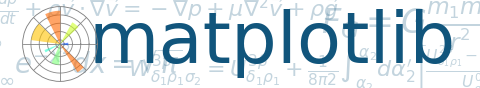
\includegraphics[width=0.9\textwidth]{im/matplotliblogo}
        %\caption{$\mu$-Penalization case}
        \label{fig::matplotliblogo}
\end{figure}
\end{frame}

\begin{frame}[fragile]{Graphique simple}

La syntaxe est très simple pour faire un graphique.

\begin{lstlisting}[language=Python]
import numpy as np
import matplotlib
import matplotlib.pyplot as plt

x=np.linspace(0,2*np.pi,100)
xx=np.linspace(0,2*np.pi,10)
alpha=1.
plt.plot(x,np.sin(alpha*x),label="$\sin(\\alpha x)$")
plt.plot(xx,np.sin(alpha*xx),"s",label="$\sin(\\alpha x)$")
plt.plot(x,np.cos(alpha*x),label="$\cos(\\alpha x)$")
# Make the legend appear
plt.legend()
# Render the plot
plt.show()
\end{lstlisting}

\end{frame}


\begin{frame}[fragile]{Graphique en échelle logarithmique}

\begin{lstlisting}[language=Python]
import numpy as np
import matplotlib
import matplotlib.pyplot as plt

dx=np.array([0.1,0.02,0.01,0.005])
error= 0.5*dx**2
a,b = np.polyfit(np.log(dx),np.log(error),1)

fig = plt.figure()
ax = fig.add_subplot(111) 
ax.plot(dx,error,'ko',label='$\Vert e_{\mathbf{u}}\Vert_{2}$')

ax.plot(dx,np.exp(b)*dx**a,'-k',label='$\Vert e_{\mathbf{u}}\Vert_{2}=%3.2f  \Delta x^{%3.2f}$' %(np.exp(b),a))

ax.set_yscale('log')
ax.set_xscale('log')

\end{lstlisting}
\end{frame}

\begin{frame}[fragile]{Graphique en échelle logarithmique - suite }

\begin{lstlisting}[language=Python]
ax.grid(b=True, which='minor', color='grey', linestyle='--')
ax.grid(b=True, which='major', color='k', linestyle='-')
plt.ylabel('$\Vert e \Vert_2 $')
plt.xlabel('$\Delta x$')
plt.legend()
plt.show()
\end{lstlisting}

\end{frame}

\section{Calcul scientifique}

\begin{frame}
\frametitle{Calcul scientifique : Le module numpy}
Le module Numpy est ce qui permet à Python d'effectuer des calculs reliés à l'algèbre linéaire : 
\begin{itemize}
    \item Création de vecteurs et matrices
    \item Opérations mathématiques sur les vecteurs et matrices
    \item Résolution de systèmes linéaires
    \item etc.
\end{itemize}
Le module Scipy est compagnon au module Numpy. Il contient quand à lui des routines complexes pour l'intégration, l'interpolation et etc.

\end{frame}


\begin{frame}[fragile]
\frametitle{Résolution d'un système linéaire}
\begin{lstlisting}[language=Python]
import numpy as np
import matplotlib
import matplotlib.pyplot as plt
n=20
dx=1/(n-1)
mat = -2*np.eye(n)
mat.flat[1::n+1]=1
mat.flat[n::n+1]=1
mat[0,:]=0
mat[-1,:]=0
mat[0,0]=1
mat[-1,-1]=1
b = - 20*np.ones(n) * dx**2.
b[0]=1
b[-1]=2
T=np.linalg.solve(mat,b)
plt.plot(np.linspace(0,1,n),T)
plt.show()
\end{lstlisting}
\end{frame}


\begin{frame}[fragile]
\frametitle{Integration numerique }
On souhaite souvent faire le post-traitement de donnée et calculer une intégrale en utilisant par exemple, la méthode des trapèze...

\begin{lstlisting}[language=Python]
import numpy as np
from scipy.integrate import simps

def f(x):    
    return x**2.

x=np.linspace(0,1,11)
# x est maintenant [0, 0.01, 0.02,...,1.]
y = f(x)
integral=np.trapz(y,x) # methode du trapeze
integralS=simps(y,x) # methode de Simpson
print("L'integrale trapz : ",integral )
print("L'integrale simps : ",integralS )
print("La solution : ", 1./3.)

\end{lstlisting}
\end{frame}

\begin{frame}[fragile]
\frametitle{Interpolation}
\begin{lstlisting}[language=Python]
import numpy as np
from scipy.interpolate import interp1d
import matplotlib.pyplot as plt

x = np.linspace(0, 10, num=11, endpoint=True)
y = np.cos(x)
f = interp1d(x, y)
f2 = interp1d(x, y, kind='cubic')
 
xnew = np.linspace(0, 10, num=41, endpoint=True)

plt.plot(x, y, 'o', xnew, f(xnew), '-', xnew, f2(xnew), '--')
plt.legend(['data', 'linear', 'cubic'], loc='best')
plt.show()


\end{lstlisting}
\end{frame}

\begin{frame}[fragile]
\frametitle{Régression linéaire}
\begin{lstlisting}[language=Python]
import numpy as np
import matplotlib.pyplot as plt
from scipy import stats

np.random.seed(12345678)
x = np.random.random(10)
y = np.random.random(10)
# Regression  polynomiale,
a,b = np.polyfit(x,y,1)
# Regression lineaire avec statistique
slope, intercept, r_value, p_value, std_err = stats.linregress(x, y)
print("r-squared:", r_value**2)
print("p-value:", p_value)
print("std_err:", std_err)
plt.plot(x,y,'o')
plt.plot(x,slope*x+intercept)
plt.show()

\end{lstlisting}
\end{frame}


\section{Calcul symbolique}

\begin{frame}
\frametitle{Calcul symbolique : Le module Sympy}
Le module Sympy permet de faire du calcul symbolique avec Python. On peut donc s'en servir comme un équivalent de Maple ou Mathematica.

Le module sympy n'est pas par défaut installé sur les jupyter notebook virtuels. Vous pouvez l'essayer en temps réel en allant sur le site: \url{http://live.sympy.org/}
\end{frame}

\begin{frame}[fragile]
\frametitle{Utilisation du calcul symbolique}
\begin{lstlisting}[language=Python]
from sympy import *

#variables symboliques
x,y = symbols("x y")
expr = cos(x) + 1

#L'operateur substitution permet de remplacer un symbole par une autre ou par une value numerique
expr.subs(x,1.)
expr.subs(x,y)

# On peut aussi definir une formule par un "string"
str_expr = "x**2 + 3*x - 1/2"
expr2 = sympify(str_expr)
expr2
\end{lstlisting}
\end{frame}

\begin{frame}[fragile]
\frametitle{Derivation symbolique}
\begin{lstlisting}[language=Python]
from sympy import *

#variables symboliques
x,y,a = symbols("x y a")

def laplacian(u):
	return diff(u,x,x)+diff(u,y,y)

u=sin(a*x)*cos(a*y)
laplacian(u)
\end{lstlisting}
\end{frame}

\begin{frame}[fragile]
\frametitle{Intégration symbolique}
\begin{lstlisting}[language=Python]
from  sympy import *

#define symbolic variables
x,y,a = symbols("x y a")

u=sin(x)*exp(x)
#Integrale symbolique sans borne
integrate(u,x)

#Integrale symbolique avec bornes
v=exp(-x)
integrate(v,(x,0,oo))
\end{lstlisting}
\end{frame}




\section{Manipulation de fichiers}

\begin{frame}
\frametitle{Manipulation de dossier et fichiers : Les modules systèmes et OS}
Les modules os et sys permette d'intéragir avec le système d'exploitation (peu importe ce qu'il soit) afin de modifier des fichiers, lancer des programmes, etc.

Ceci permet de remplacer totalement l'usage de bash pour automatiser la soumission de tâches, les études paramétriques, etc.

Dans ce qui suit, nous verrons des exemples simples d'utilisation.
\end{frame}

\begin{frame}[fragile]
\frametitle{Passage d'argument à un script python}
Les scripts python peuvent prendre des argument en ligne de commande:
\begin{lstlisting}[language=Python]
import sys


for i in sys.argv:
	#sys.argv contient toujours un argument, c'est a dire le nom du fichier python
	print i



\end{lstlisting}
\end{frame}

\begin{frame}[fragile]
\frametitle{Manipulation de dossiers }
Le module os permet la naviguation et manipulation de dossiers
\begin{lstlisting}[language=Python]
import os

path="/home/blab/"
#Affiche le contenu du dossier
os.listdir(path)

#Change de dossier
os.chdir

for i in sys.argv:
	#sys.argv contient toujours un argument, c'est a dire le nom du fichier python
	print i



\end{lstlisting}
\end{frame}

\begin{frame}[fragile]
\frametitle{Lancement d'un programme externe}
Le module os permet de lancer des programmes externes et de récupérer le status d'exécution du programme.
\begin{lstlisting}[language=Python]
import os
retour=os.system("./testapp.sh")   
# si l'application se termine bien alors retour vaudra 0
# sinon retour vaudra le statut d'erreur 
\end{lstlisting}

\end{frame}

\begin{frame}[fragile]
\frametitle{Remplacement dans un ficher texte}
Python permet l'utilisation d'expression régulières à partir du module re. Le code suivant permet de faire l'équivalent d'un sed dans un fichier texte simplement et efficacement.
\begin{lstlisting}[language=Python]
import re
with open("./fichier", "r") as sources:
    lines = sources.readlines()
with open("./output", "w") as sources:
    for line in lines:
        sources.write(re.sub(r'ours', 'canard', line))
        
\end{lstlisting}
\end{frame}


 
\end{document}

